\section{Results}
\subsection{results of single models}
Before merging the three models together it must be controlled whether each model is implemented correctly for itself. The pictures of the models simulation results are the guide for this. Sometimes there are discrepanies between the puplished model and the picture which should represent the model.  Hereafter, the implementation process for each of the models is described.

\subsubsection{Ion model}
The challanges with the implementation of the ion model where, that the presented equation, initial values and parameters did not result in the intended system behaviour. \\
After an in-depth analysis of the equation there where two anomalies:

\begin{enumerate}
	\item the calculation of the change of the inner proton ion concentration has \emph{Bf} as an undefined parameter
	\item the fluxes have the wrong units
\end{enumerate}
For solving the problem with the undefined parameter in (1) the ODE was constructed by deriving the formula for the calculation of the pH value for diluted solution 

\begin{equation*}
pH = - log_{10}([H^+])
\frac{d}{dt} pH = - \frac{d}{dt} log_{10}([H^+])
= - \frac{1}{ln(10)} \frac{d}{dt}ln([H^+])
\end{equation*}

The published ion model has discrepancies in the parameter values of the phenomenological and stoichiometric coefficients and the calculation of the ion fluxes have the wrong units \\\\
The ion model assumes that the celllular compartment and the environment are well mixed. Their does not exists concentrations gradients. \\\\
\begin{figure}[htbp]
	
	\begin{minipage}{0,5\textwidth}
		
		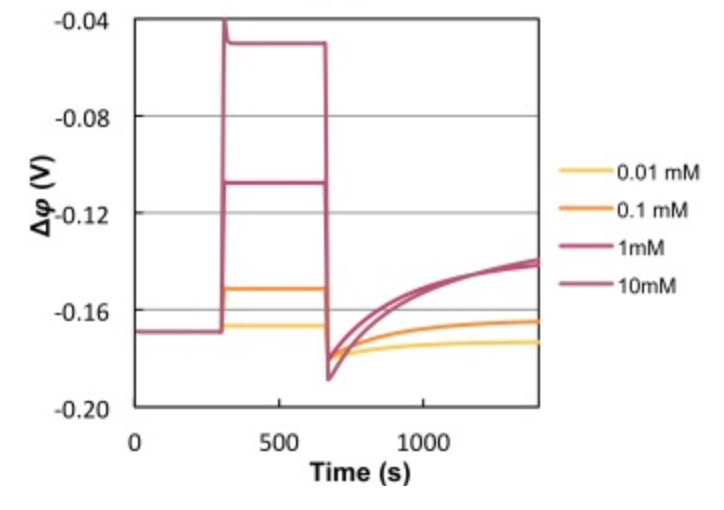
\includegraphics[width=\textwidth]{picture/Ion_Paper.png}
		
		\label{IonPaper} 
	\end{minipage}
	\begin{minipage}{0,5\textwidth}
		
		\includegraphics[width=\textwidth]{picture/ion_examine.png}
		
		\label{IonImplemented} 
	\end{minipage}
	\caption{left: membrane voltage in the ion paper for different NaCl stimulus (0.01 mM - 10 mM); right: the simulated implemented ion model for the same stimulus range }
\end{figure}

\subsection{hog model}
The hog model consists of ODEs of the following form:
\begin{equation}\label{VratioChange}
	\frac{d[P]}{dt} = f(\vec{P})-V_{ratio}\cdot [P]
\end{equation}

Equation \ref{VratioChange} describes in general  with the first term at the right hand side the changes of a concentration due to a chemical process and with the second term the changes in the concentration due to changes in volume \cite{Ke_2013}.\\

\begin{figure}[htbp]
	
	\begin{minipage}{0,5\textwidth}
		
		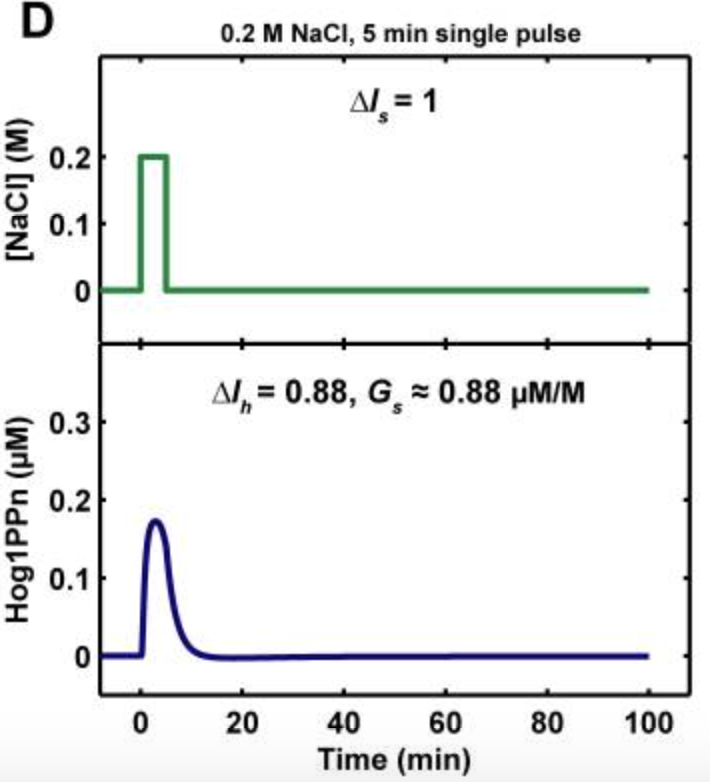
\includegraphics[width=\textwidth]{picture/Hog_Paper.png}
		
		\label{IonPaddper} 
	\end{minipage}
	\begin{minipage}{0,5\textwidth}
		
		\includegraphics[width=\textwidth]{picture/hog_examine.png}
		
		\label{IonImpdlemented} 
	\end{minipage}
	\caption{left below: membrane voltage in the ion paper for different NaCl stimulus (0.01 mM - 10 mM); right: the simulated implemented ion model for the same stimulus range }
\end{figure}

\subsection{volume model}
\begin{figure}[htbp]
	
	\begin{minipage}{0,5\textwidth}
		
		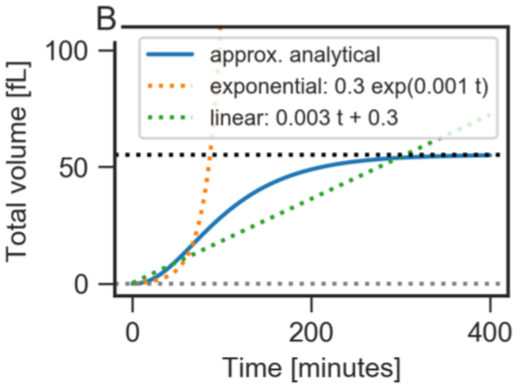
\includegraphics[width=\textwidth]{picture/Volume_Paper.png}
		
		\label{IonPadper} 
	\end{minipage}
	\begin{minipage}{0,5\textwidth}
		
		\includegraphics[width=\textwidth]{picture/volume_examine.png}
		
		\label{IonImpledmented} 
	\end{minipage}
	\caption{left: membrane voltage in the ion paper for different NaCl stimulus (0.01 mM - 10 mM); right: the simulated implemented ion model for the same stimulus range }
\end{figure}


\subsection{merging of the models}
The process of merging models is a tricky task. There exists some good guideline \cite{Liebermeister2008ValidityAC} for this.
Hereafter, the used essential steps are sketched:
\begin{enumerate}
	\item equations: One of the first steps in the process of model merging is the control whether there is a conflict between assumptions of the description of the biological systems. Conflicts must be resolved by combining equation terms or discard some informations
	\item names: Find all the overlaps in the variable and parameter naming and convert them to a common sets of names
	\item units: Standardize all used units for the parameter and initial values to a common set. In this process new factors where give to individual values if the unit changes requires that.
\end{enumerate}
Changes in the equation design (ODE and algebraic equation) in the process of merging the model were done and are presented below:
\begin{table} [h]
	\footnotesize
\begin{center} 
	\caption{changes in the equation design}
\begin{tabular} {l l l l l l l l}
%&  \multicolumn{2}{c}{changing equation}  \\ \hline
& changes & reason\\
internal / external osmolyt concentration & $c = \sum ([Ionen]+[other osmolyte])$ & simplification\\ 
internal / external presure & $\pi = c \cdot R \cdot T	$ & simplification\\
ion x changes & $\frac{J_x \cdot CellSurface}{CellVolume} \cdot 10^{6}$ & unit harmonization\\
sorbitol stimulus & $\frac{d}{dt}[Sorbitol]=0$ & implementation of sorbitol stimulus with the assumation that sorbitol can not diffuse over the plasma membrane; in ODE format because due to the simulation design this approach results in less memory data\\
uptake / dilution of osmotically active compounds & removed & replaced with the equation for the ion and glycerol
\end{tabular}
\label{changesOnTheModels}
\end{center}
\end{table}

In the whole process of merging we must consider their biochemical interpretation to maintain the plausblity of the model \cite{Liebermeister2008ValidityAC}. No parameter value was changed in his biological interpretation.\\\\

Initial values were changed because as we can see in \ref{IntersectionsOfTheModels} multiple components are used in several models. The components have different quantities in the initial assumptions. One of the main difference was the assumption of the cell volume $V_cell$ in the hog model ($V_{cell}=58fL $) and the volume model ($V_{cell} \approx 0.27fL$). To solve this problem we simulated the volume model until $V_cell$ also have the value of $58fL$. We assumed the ODE values at this time point as the initial values for the corresponding substance in the merged model. \\\\

\subsection{combined model}
For the analysis and validation of the merged model we choosed the nuclear phophorylated Hog1 (Hog1PPn) as the control substance. Hog1PPn is also used in the hog model as the output because it regulates the expression of hundred of genes \cite{Zi_2010}. We borrowed the idea of a drug response curve from the theme field pharmocokinetic (zitieren: hier das Buch!!!) as a visualized output showed below.  \\
(hier noch das falsche Bild, da Simulation noch nicht ganz fertig)
\begin{figure}[h!]
	\begin{center}
		\begin{minipage}{0,8\textwidth}
			
			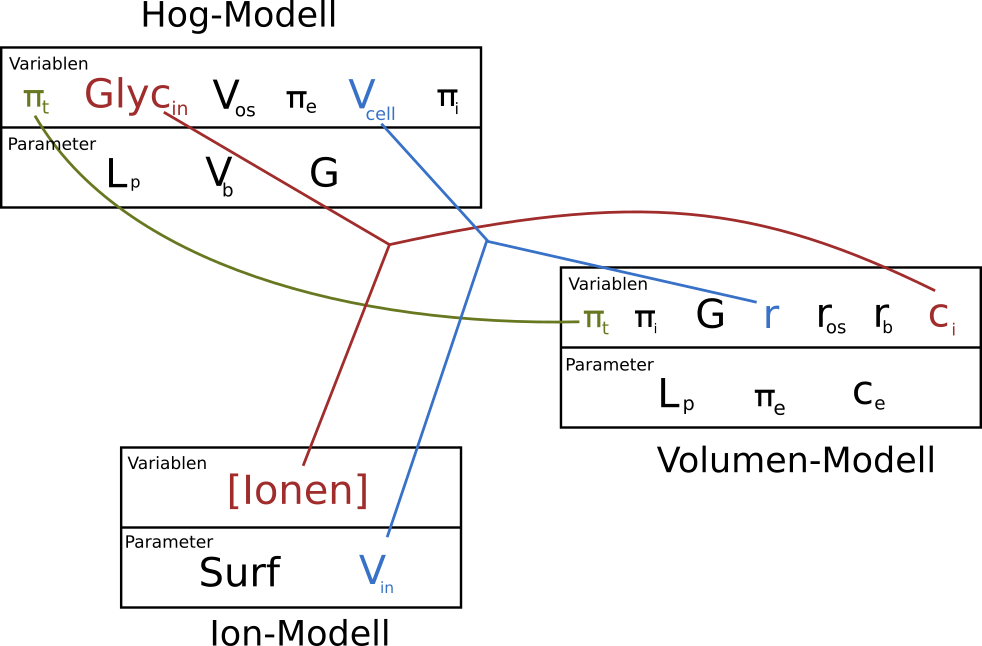
\includegraphics[width=\textwidth]{picture/model_intersections.png}
			\caption{Response of Hog1PPn} 
			\label{DrugResponseCurve} 
		\end{minipage}
	\end{center}
\end{figure}

\subsubsection{single models with the initial values from the combined model}
After implement the initial values from the combined model back to the single models, no difference for the hog model was simulated. The reason for this lays in the simple reason, that we only changed the initial values from the ion and the volume model in the combined model.\\
The problem for compering the simulation results for the volume model is the fact, that the original data from the Github-Account of the ...

\newpage
